A model transformation $\MT\colon \Lang(D_1) \TransMT \Lang(D_2)$ is specified by a TGG (cf. \cref{sec-gen-intro-mt}).
In the following we review the existing concept of executing model transformations from \cite{FAGT2} based on model transformation sequences via operational rules of a given TGG, called forward translation triple rules.
According to \cref{def:sec-mt-tgg:fwd_bwd_tr_rules}, the operational forward translation rules of a given TGG are derived from the set of triple rules of the TGG by an automatic construction \cite{DBLP:conf/gg/SchurrK08,Hermann:2010:EAE:1866272.1866277}.
For each triple rule $\tr$, the construction yields a corresponding forward translation triple rule $\tr_\FT$ which is identical to $\tr$ on the correspondence and target components, i.e., $\tr_\FT$ creates the same graph elements as $\tr$ in the correspondence and target parts.
For the source part, $\tr_\FT$ does not create elements but already contains the created source elements of $\tr$ in the left-hand side.
Each source graph element in $\tr_\FT$ is equipped with a translation attribute with attribute value false ($\False$ - not yet transformed) for those elements that are created by $\tr$ and attribute value true ($\True$ - has been already transformed) for all other elements (cf. \cref{rem:sec-mt-tgg:tr_attr}).
Therefore, the application of a forward translation rule $\tr_\FT$ is the transformation of all source elements that are marked with $\False$ to corresponding target elements.
Furthermore, rule $\tr_\FT$ updates all translation attribute values from $\False$ to $\True$ in order to mark that the corresponding elements has been transformed.
According to \cref{def:sec-mt-tgg:mt_ft}, a forward model transformation is executed by applying operational forward translation rules successively in so called model transformation sequences.
Thus, the execution of a model transformation corresponds to the abstract description in \cref{sec-gen-intro-gratrafo} where the update of the translation attribute values from $\False$ to $\True$ corresponds to the marking of graph elements to keep track of the elements that already have been transformed during the execution.
The backward case of transforming models from $\Lang(D_1)$ in source domain $D_1$ to $\Lang(D_2)$ in target domain $D_2$ via backward translation rules is defined analogously and omitted in the following.
For technical details we refer to Chapter 7 in \cite{FAGT2}.

The extension of rules with translation attributes from \cref{rem:sec-mt-tgg:tr_attr} is used for the definition of forward translation rules in \cref{def:sec-mt-tgg:fwd_bwd_tr_rules} and for the definition of marking rules in \cref{sec-dc-verification} that are part of verifying domain completeness.

\begin{remark}[Graphs with Translation Attributes]
\label{rem:sec-mt-tgg:tr_attr}
Given an attributed graph $\AG=(G,D)$ and a subset $M \subseteq G$ of its elements (nodes, edges or attributes), we call \emph{$\AG'$ a graph with translation attributes over $\AG$}\index{graph!with translation attributes} if it extends $\AG$ by one Boolean-valued translation attribute for each element in $M$.
The translation attribute for a node or edge is specified by an attribute $\tr$.
The translation attribute for an attribute $a$ of a node or edge is specified by an attribute $\tr\_a$.
With $\AG \oplus \Att^\True_M$ we denote the graph with translation attributes over $\AG$ which extends $\AG$ by a translation attribute for each element in $M \subseteq G$, and all these translation attributes are set to $\True$.
Similarly, $\AG \oplus Att^\False_M$ denotes adding to $\AG$ all these translation attributes, but this time they are set to $\False$.
With $\Att^x(\AG),x \in \{\False,\True\}$ we denote $\AG \oplus \Att^x_G$.
For technical details we refer to Sec. 7.4.1 in \cite{FAGT2}.
\envEndMarker
\end{remark}

According to \cref{def:sec-mt-tgg:T-Ext}, for forward translation rules with application conditions $\ac$, each element in $\ac$ that is not in the premise of $\ac$ also need to be extended by a translation attribute of value $\True$.
For triple rules, $X$ restricts the extension to elements of specific triple components (source, correspondence and target).

\begin{definition}[$\True$-Extension of Application Conditions (Def. 7.28 in \cite{FAGT2})]
\label{def:sec-mt-tgg:T-Ext}
\index{application condition!$\True$-Extension}
Given an application condition $\ac_P$ over premise graph $P$, a graph $P'$ with translation attributes over $P$ and a subset of triple components $X \subseteq \{S,C,T\}$, then the $\True$-extension $tExt(\ac_P,P',X)$ of $\ac_P$ is inductively defined by:
\begin{itemize}
  \item $\tExt(\true,P',X)=\true$
  \item $\tExt(\exists(a=(\inc_P,a_D)\colon P \to C, \ac_C),P',X)=\exists(a_E\colon P' \to C',\tExt(\ac_C,C',X))$ with
  \begin{enumerate}
    \item $C'=P' +_P C \oplus \cup_{x \in X}(\Att^\True_{C^x\setminus P^x})$, and
    \item $a_E=(\inc'_P,a_D)$ with algebra homomorphism $a_D$ on the data part and inclusion $\inc'_P$ on the graph part as derived from $\inc_P$.
  \end{enumerate}
\item $\tExt(\neg(\ac'_P),P',X)=\neg(\tExt(\ac'_P,P',X))$
  \item $\tExt(\ac_{P,1} \wedge \ac_{P,2},P',X)=\tExt(\ac_{P,1},P',X) \wedge \tExt(\ac_{P,2},P',X)$
  \item $\tExt(\ac_{P,1} \vee \ac_{P,2},P',X)=\tExt(\ac_{P,1},P',X) \vee \tExt(\ac_{P,2},P',X)$
  \envEndMarker
\end{itemize}
\end{definition}

According to \cite{FAGT2}, for model transformations and synchronisations, we restrict the application conditions of triple rules to $S$-consistent application conditions.

\begin{remark}[$S$-consistent Application Conditions]
\label{rem:sec-mt-tgg:s_consistent}
According to Def. 7.8 in \cite{FAGT2}, an application condition $\ac_P$ is source consistent ($S$-consistent)\index{application condition!$S$-consistent}, if it can be decomposed into a semantically equivalent conjunction $\ac_P \equiv \ac_S \wedge \ac_F$ such that $\ac_S$ does restrict the source component only and $\ac_F$ does restrict the correspondence and target components only, i.e., relations of restricting elements between the correspondence and source parts in $\ac_P$ may be problematic.
All application conditions in running examples of this thesis are $S$-consistent.
\envEndMarker
\end{remark}

Forward translation rules are used in \cref{def:sec-mt-tgg:mt_ft} for executing model transformations and in \cref{sec-dom-compl-mt,thm:sec-dom-compl-mt-without-acs} for verifying the domain completeness of model transformations.

\begin{definition}[Forward Translation Rule (Def. 7.29 in \cite{FAGT2})]
\label{def:sec-mt-tgg:fwd_bwd_tr_rules}
Given a triple rule $\tr=((\tr^\SRC,\tr^\C,\tr^\T)\colon L=(L^\SRC \transB{s_L} L^\C \trans{t_L} L^\T) \to R=(R^\SRC \transB{s_R} R^\C \trans{t_R} R^\T),\ac_L)$ with $S$-consistent application condition $\ac_L$ over $L$, then \emph{the forward translation rule $\tr_\FT$ of $\tr$}\index{triple rule!forward translation rule} is given by $\tr_\FT=(L_\FT \transB{l_\FT} K_\FT \trans{r_\FT} R_\FT,\ac_\FT)$ with:
\begin{enumerate*}
  \item $L_\FT=(R^\SRC \transB{\tr^\SRC \circ s_L} L^\C \trans{t_L} L^\T) \oplus \Att^\True_{(\tr^\SRC(L^\SRC) \gets \varnothing \to \varnothing)} \oplus \Att^\False_{(R^\SRC \gets \varnothing \to \varnothing) \setminus (\tr^\SRC(L^\SRC) \gets \varnothing \to \varnothing)}$,
  \item $K_\FT=(R^\SRC \transB{\tr^\SRC \circ s_L} L^\C \trans{t_L} L^\T) \oplus \Att^\True_{(\tr^\SRC(L^\SRC) \gets \varnothing \to \varnothing)}$,
  \item $R_\FT=(R^\SRC \transB{s_R} R^\C \trans{t_R} R^\T) \oplus \Att^\True_{(R^\SRC \gets \varnothing \to \varnothing)}$,
  \item $l_\FT$ and $r_\FT$ are the induced inclusions, and
  \item $\ac_\FT=\tExt(\ac_L,L_\FT,\{S\})$.
\end{enumerate*}
With $\TR_\FT$ we denote the set of forward translation rules $\tr_\FT$ of all triple rules $\tr \in \TR$ for a given set of triple rules $\TR$.
\envEndMarker
\end{definition}

\begin{definition}[Complete Forward Translation Sequence (Def. 7.33 in \cite{FAGT2})]
\label{def:sec-mt-tgg:compl_ft}
A forward translation sequence $G_0 \Trans{\tr^*_{\FT}} G_n$ via $\TR_\FT$ with almost injective matches is \emph{complete}\index{model transformation!forward translation sequence}, if no further forward translation rule is applicable and all translation attributes in $G_n$ are set to $\True$.
\envEndMarker
\end{definition}

\begin{definition}[Model Transformation based on Forward Translation Rules (Def. 7.34 in \cite{FAGT2})]
\label{def:sec-mt-tgg:mt_ft}
Given a triple type graph $\TG=(\TG^\SRC \gets \TG^\C \to \TG^\T)$ and a set $\TR$ of triple rules typed over $\TG$, then a \emph{model transformation sequence}\index{model transformation!sequence} $(G^S,G'_0 \Trans{\tr^*_{\FT}} G'_n,G^T)$ based on forward translation rules $\TR_{\FT}$ from a source graph $G^S$ in the source domain to a target graph $G^T$ in the target domain consists of a complete forward translation sequence $G'_0 \Trans{\tr^*_{\FT}} G'_n$ typed over $\TG'=\TG \oplus \Att^\False_{(\TG^S \gets \varnothing \to \varnothing)} \oplus \Att^\True_{(\TG^S \gets \varnothing \to \varnothing)}$ based on $\TR_{\FT}$ with $G'_0=(\Att^\False(G^S) \gets \varnothing \to \varnothing)$ and $G'_n=(\Att^\True(G^S) \gets G^C \to G^T)$.
A \emph{model transformation}\index{model transformation} $\MT\colon \Lang(\TG^S) \TransMT \Lang(\TG^T)$ based on $\TR_{\FT}$ is defined by all model transformation sequences as above with $G^S \in \Lang(\TG^S)$ and $G^T \in \Lang(\TG^T)$ (cf. \cref{sec-dc-general,def:sec-dc-general:lang} for $\Lang(\TG^\SRC)$ and $\Lang(\TG^\T)$).
\envEndMarker
\end{definition}

\begin{figure}[!tb]
\begin{center}
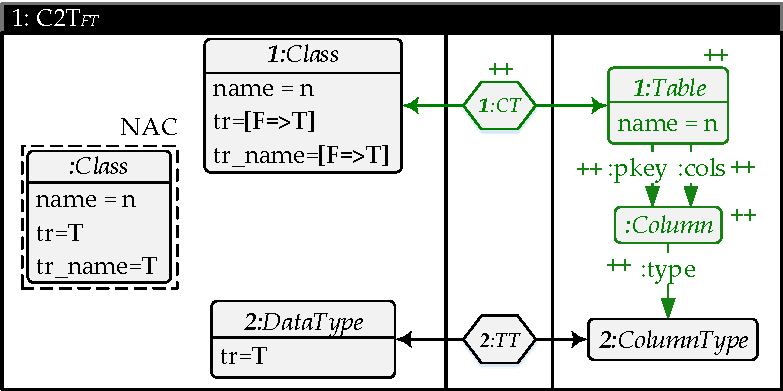
\includegraphics[width=.7\textwidth]{img/gen_intro/ft.pdf}
\end{center}
\caption{Forward Translation Rule}
\label{fig:sec-mt-tgg:fwd_tr_rule}
\end{figure}

\begin{example}[Forward Translation Rule \& Model Transformation]
\label{ex:sec-mt-tgg:fwd_mt}
Rule \code{C2T}$_\FT$ in \cref{fig:sec-mt-tgg:fwd_tr_rule} is the forward translation rule of triple rule \code{C2T} in \cref{sec-gt-trafo,fig:sec-gt-trafo:tgg}.
Node \code{1:Class} and attribute \code{name} are created by rule \code{C2T} in the source and therefore, are initially marked with translation attribute $\False$ and updated to $\True$ in rule \code{C2T}$_\FT$, denoted by $[\False => \True]$.
All other source and NAC elements of \code{C2T} are initially marked with $\True$ in \code{C2T}$_\FT$ and remain unchanged.
Furthermore, the correspondence and target components of \code{C2T}$_\FT$ are identical to those of rule \code{C2T}.
Note that a forward translation rule does also contain the application condition of the target component but without any markings if existent in the underlying triple rule as it is the case for triple rules \code{TD2T} and \code{TC2T}.
Graph $\CD$ in \cref{sec-gt-graphs,fig:sec-gt-graphs:atg} can be transformed to graph $\RDBM$ via model transformation sequence $(\CD,G'_0 \Trans{\code{DT2CT}_\FT(``INT'')} G'_1 \Trans{\code{C2T}_\FT(``Person'')} G'_2 \Trans{\code{A2C}_\FT(``DOB'')} G'_3 \Trans{\code{MC}_\FT} G'_4 \Trans{\code{TD2T}_\FT} G'_5,\RDBM)$ based on the forward translation rules of the triple rules in \cref{sec-gt-trafo,fig:sec-gt-trafo:tgg} with integrated model $G'_5=(\Att^\True(\CD) \gets G^\C \to \RDBM)$.
The model transformation CD2RDBM is given by all corresponding model transformation sequences based on the forward translation rules of the triple rules in \cref{sec-gt-trafo,fig:sec-gt-trafo:tgg}.
\envEndMarker
\end{example}

\paragraph*{General Assumption}
\label{rem:sec-mt-tgg:gen_ass}
Note that the definition of forward translation rules is based on attributions in attributed graphs (cf. \cref{rem:sec-mt-tgg:tr_attr,def:sec-mt-tgg:fwd_bwd_tr_rules}).
Therefore, we assume category $(\ATrGraphs_\ATGI,\M)$ for model transformations and synchronisations.
According to the general assumption for model transformations based on TGGs in Sec. 7.1 in \cite{FAGT2} and analogously to the general assumption for rule applications in \cref{sec-gt-trafo}, we assume that triple rules are applied based on transformations via almost injective matches $m \in \morO$ and where all internal morphisms of application conditions are almost injective (cf. \cref{sec-tgg} for $\morO$-morphisms in $(\ATrGraphs_\ATGI,\M)$).
In the context of model transformations and synchronisations, we generally assume the empty triple graph $\varnothing$ as start graph for TGGs and that all application conditions of triple rules are $S$-consistent.
